\documentclass{article}
\usepackage{tikz}
\usetikzlibrary{positioning, arrows.meta}
\usepackage[margin=0.5in]{geometry} % optional: smaller margins

\begin{document}

\begin{figure}[h!]
\centering
\resizebox{\textwidth}{!}{%
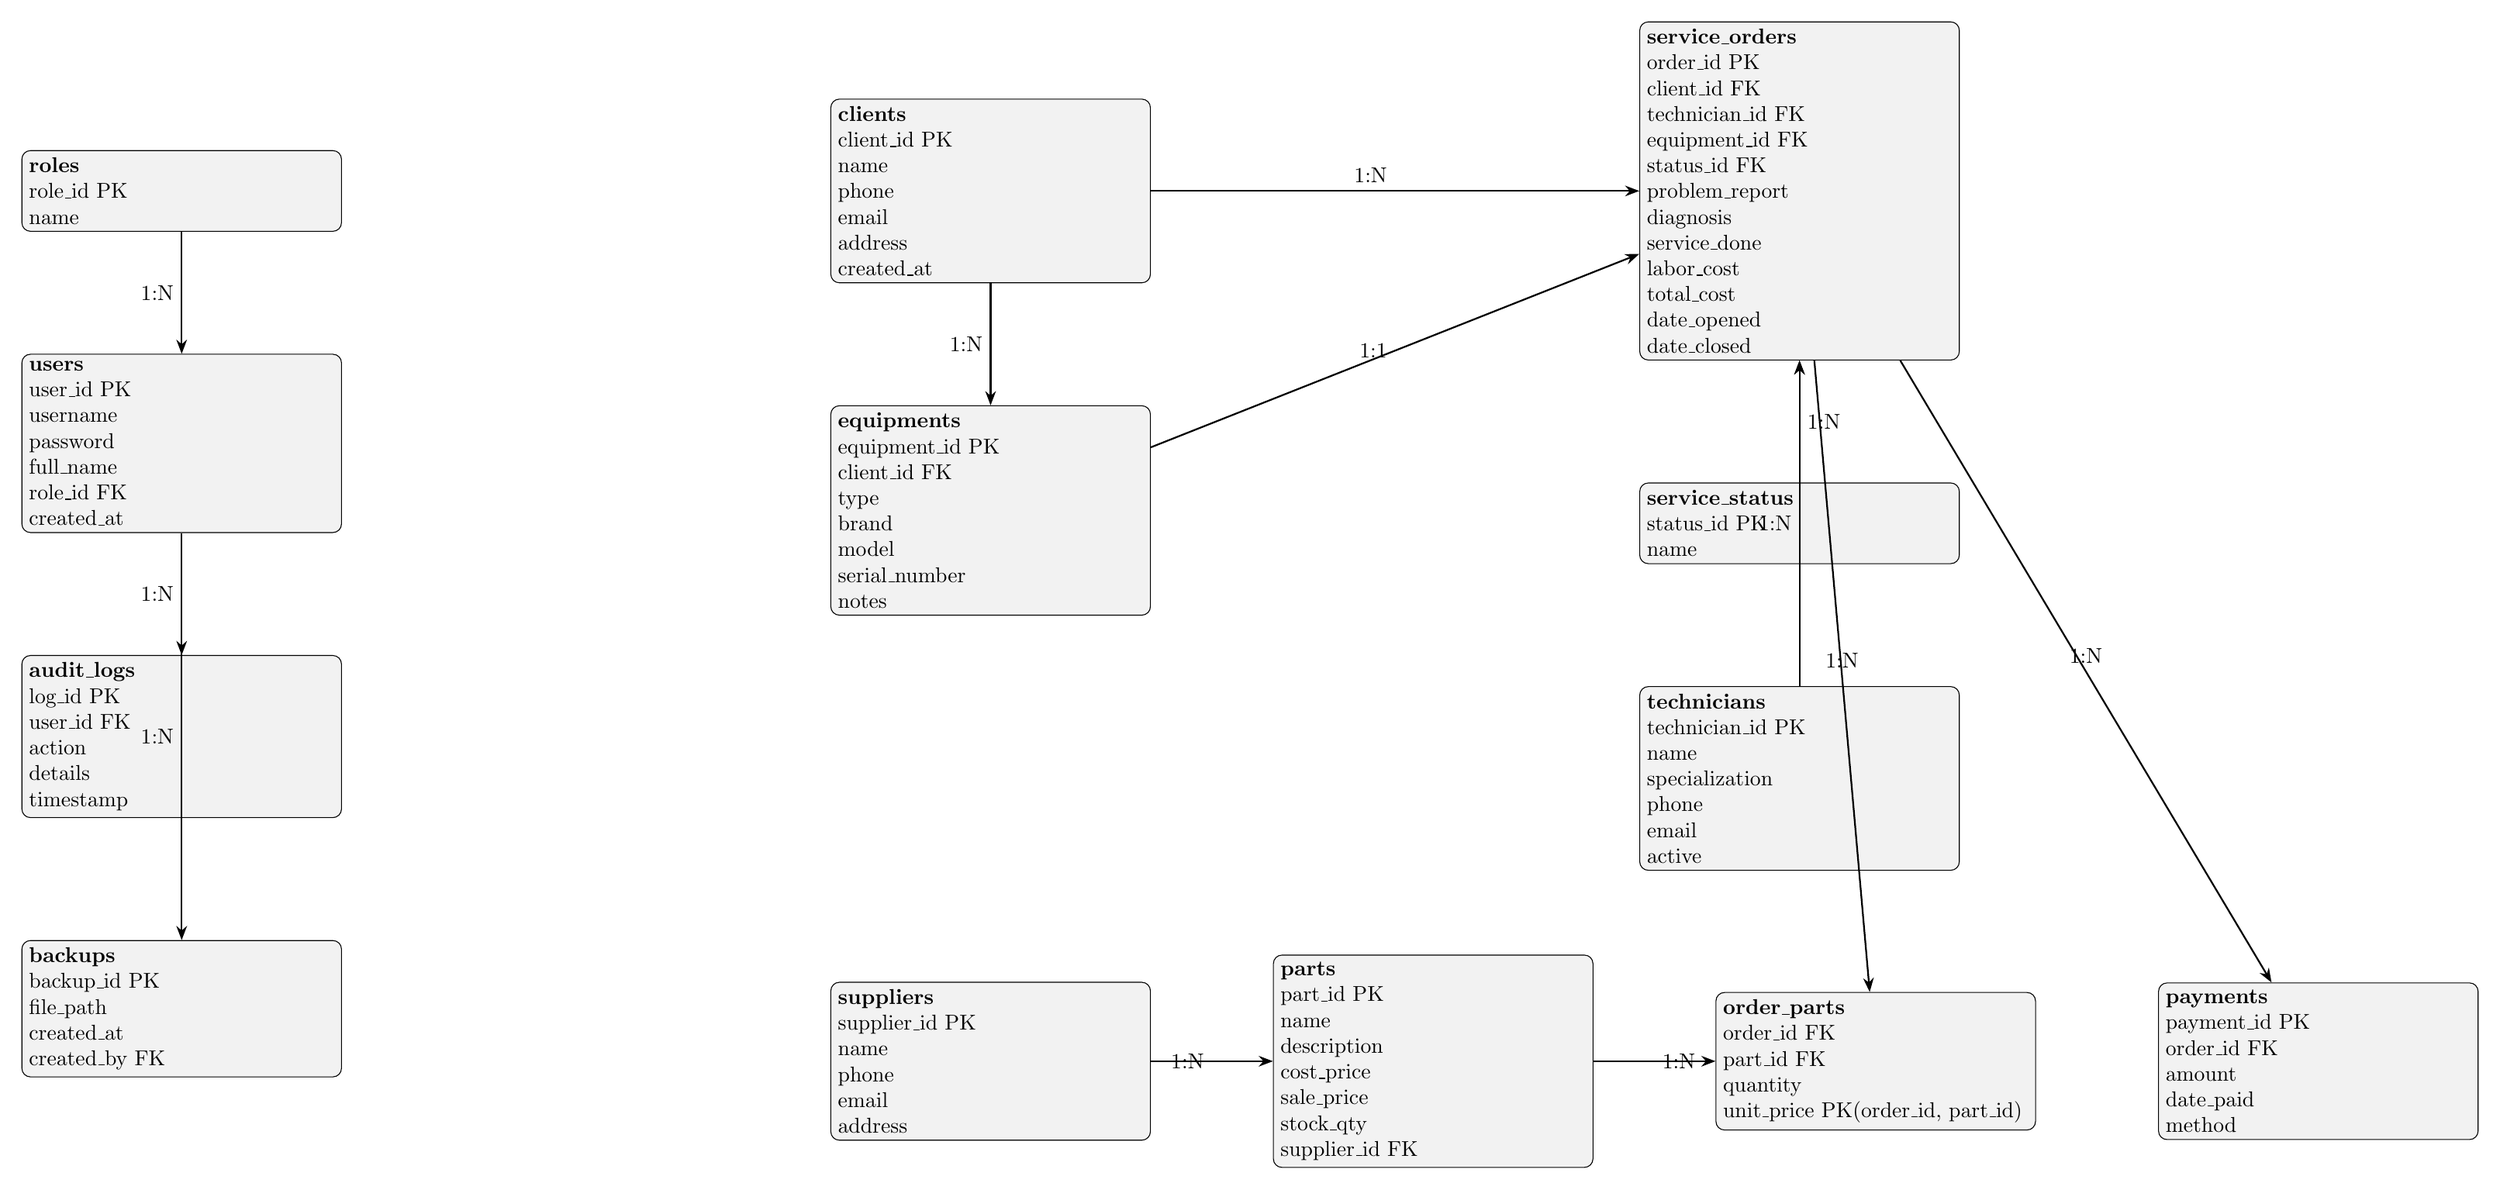
\begin{tikzpicture}[
  table/.style={rectangle, draw=black, fill=gray!10, text width=5cm, minimum height=1cm, align=left, rounded corners},
  rel/.style={-{Stealth}, thick, bend left=10},
  node distance=2cm
]

% ======================
% AUTHENTICATION
% ======================
\node[table] (roles) {
\textbf{roles}\\
role\_id PK\\
name
};

\node[table, below=of roles] (users) {
\textbf{users}\\
user\_id PK\\
username\\
password\\
full\_name\\
role\_id FK\\
created\_at
};

\node[table, below=of users] (audit_logs) {
\textbf{audit\_logs}\\
log\_id PK\\
user\_id FK\\
action\\
details\\
timestamp
};

\node[table, below=of audit_logs] (backups) {
\textbf{backups}\\
backup\_id PK\\
file\_path\\
created\_at\\
created\_by FK
};

% ======================
% CLIENTS & EQUIPMENTS
% ======================
\node[table, right=of roles, xshift=6cm] (clients) {
\textbf{clients}\\
client\_id PK\\
name\\
phone\\
email\\
address\\
created\_at
};

\node[table, below=of clients] (equipments) {
\textbf{equipments}\\
equipment\_id PK\\
client\_id FK\\
type\\
brand\\
model\\
serial\_number\\
notes
};

% ======================
% SERVICE ORDERS
% ======================
\node[table, right=of clients, xshift=6cm] (service_orders) {
\textbf{service\_orders}\\
order\_id PK\\
client\_id FK\\
technician\_id FK\\
equipment\_id FK\\
status\_id FK\\
problem\_report\\
diagnosis\\
service\_done\\
labor\_cost\\
total\_cost\\
date\_opened\\
date\_closed
};

\node[table, below=of service_orders] (service_status) {
\textbf{service\_status}\\
status\_id PK\\
name
};

\node[table, below=of service_status] (technicians) {
\textbf{technicians}\\
technician\_id PK\\
name\\
specialization\\
phone\\
email\\
active
};

% ======================
% INVENTORY / PARTS
% ======================
\node[table, below=of equipments, yshift=-4cm] (suppliers) {
\textbf{suppliers}\\
supplier\_id PK\\
name\\
phone\\
email\\
address
};

\node[table, right=of suppliers] (parts) {
\textbf{parts}\\
part\_id PK\\
name\\
description\\
cost\_price\\
sale\_price\\
stock\_qty\\
supplier\_id FK
};

\node[table, right=of parts] (order_parts) {
\textbf{order\_parts}\\
order\_id FK\\
part\_id FK\\
quantity\\
unit\_price PK(order\_id, part\_id)
};

\node[table, right=of order_parts] (payments) {
\textbf{payments}\\
payment\_id PK\\
order\_id FK\\
amount\\
date\_paid\\
method
};

% ======================
% RELATIONSHIPS
% ======================
\draw[rel] (roles) -- (users) node[midway, left]{1:N};
\draw[rel] (users) -- (audit_logs) node[midway, left]{1:N};
\draw[rel] (users) -- (backups) node[midway, left]{1:N};

\draw[rel] (clients) -- (equipments) node[midway, left]{1:N};
\draw[rel] (clients) -- (service_orders) node[midway, above left]{1:N};
\draw[rel] (technicians) -- (service_orders) node[midway, left]{1:N};
\draw[rel] (equipments) -- (service_orders) node[midway, left]{1:1};
\draw[rel] (service_status) -- (service_orders) node[midway, right]{1:N};

\draw[rel] (suppliers) -- (parts) node[midway, left]{1:N};
\draw[rel] (parts) -- (order_parts) node[midway, right]{1:N};
\draw[rel] (service_orders) -- (order_parts) node[midway, above]{1:N};
\draw[rel] (service_orders) -- (payments) node[midway, above]{1:N};

\end{tikzpicture}%
}
\caption{Modelo Entidade-Relacionamento do SGOS (compacto e legível, TikZ puro)}
\end{figure}

\end{document}
